\documentclass{article}

\usepackage[L7x,T1]{fontenc}
\usepackage[utf8]{inputenc}
\usepackage{a4wide}
\usepackage{csquotes}
\usepackage[english]{babel}
\usepackage[maxbibnames=99,style=authoryear]{biblatex}
\addbibresource{bib.bib}
\usepackage{hyperref}
\usepackage{caption}
\usepackage{subcaption}
\usepackage{gensymb}
\usepackage{varwidth}
\usepackage{tabularx}
\usepackage{tikz}
\usetikzlibrary{er,positioning}
\input{version}

\title{
    Cartografic Generalization of Lines \\
    (example of rivers) \\ \vspace{4mm}
}

\iffalse
https://bost.ocks.org/mike/simplify/

small scale: 1:XXXXXX
large scale: 1:XXX

take douglas-pecker and check for different scales.

a4: 210x297mm
a6: 105x148xmm
a7: 74x105mm
a8: 52x74mm

connect rivers first to a single polylines:
- some algs can preserve connectivity, some not.

ideal hypothesis: mueller algorithm + topology may fully realize cartographic generalization tasks.

what scales and what distances?

https://postgis.net/docs/ST_SimplifyVW.html
https://postgis.net/docs/ST_Simplify.html
https://postgis.net/docs/ST_SimplifyPreserveTopology.html

how is tolerance bound to scale?
- just use same parameter.


\fi

\author{Motiejus Jakštys}

\date{
    \vspace{10mm}
    Version: \VCDescribe \\ \vspace{4mm}
    Generated At: \GeneratedAt
}

\begin{document}
\maketitle

\newpage

\section{Abstract}
\label{sec:abstract}

Current open-source line generalization solutions have their roots in
mathematics and geometry, thus emit poor cartographic output. Therefore, if one
is using open-source technology to create a small-scale map, downscaled lines
(e.g. rivers) will not be professionally scale-adjusted. This paper explores
line generalization algorithms and suggests one for an avid GIS developer to
implement. Once it is usable from within open-source GIS software (e.g. QGIS or
PostGIS), rivers on these small-scale maps will look professionally downscaled.

\section{Introduction}
\label{sec:introduction}

Cartographic generalization is one of the key processes of creating small-scale
maps: how can one approximate object features, without losing its main
cartographic properties? The problem is universally challenging across many
geographical entities (\cite{muller1991generalization},
\cite{mcmaster1992generalization}). This paper focuses on line generalization,
using natural rivers as examples.

Line generalization algorithms are well studied, tested and implemented, but
they expose deficiencies in large-scale reduction (\cite{monmonier1986toward},
\cite{mcmaster1993spatial}). Most of these techniques are based on mathematical
shape representation, rather than cartographic characteristics of the line.

A number of cartographic line generalization algorithms have been researched,
which claim to better process cartographic objects like lines. These fall into
two rough categories:
\begin{itemize}
    \item Cartographic knowledge was encoded to an algorithm (bottom-up
        approach). One among these are \cite{wang1998line}.
    \item Mathematical shape transformation which yields a more
        cartographically suitable down-scaling. E.g. \cite{jiang2003line},
        \cite{dyken2009simultaneous}, \cite{mustafa2006dynamic},
        \cite{nollenburg2008morphing}.
\end{itemize}

During research, code has been written for all of the algorithms above,
however, it is nowhere to be found completely, or in a usable form. There is
one exception: \cite{wang1998line} is available for general use in a commercial
product, but the author of this paper does not have means to try it.

Therefore, this paper will be comparing algorithms that readily available for
general public:
\begin{itemize}
    \item \cite{douglas1973algorithms} via
        \href{https://postgis.net/docs/ST_Simplify.html}{PostGIS Simplify}.

    \item \cite{visvalingam1993line} via
        \href{https://postgis.net/docs/ST_SimplifyVW.html}{PostGIS SimplifyVW}.
\end{itemize}

For comparison reasons, this article will be using Lakaja and large part of Žeimena
(see figure~\ref{fig:zeimena} on page~\pageref{fig:zeimena}). This location was
chosen because it is a combination of straight and curved river shape,
combination of two curly rivers, and author's familiarity with the location.

\begin{figure}
    \centering
    \includegraphics[width=148mm]{zeimena-pretty}
    \caption{Lakaja and Žeimena}
    \label{fig:zeimena}
\end{figure}

\section{Mathematical and geometrical algorithms}

As one can observe in figure~\ref{fig:douglas-300}, the Douglas \& Peucker with
300m tolerance preserves most of the shape, and 1000m
(figure~\ref{fig:douglas-1000}) is still recognizeable.

\renewcommand{\tabularxcolumn}[1]{>{\small}m{#1}}
\begin{tabularx}{\textwidth}{ p{1.5cm} | X | X }
    Tolerance          &
    Douglas \& Peucker &
    Visvalingam-Whyatt \\ \hline

    foo &
    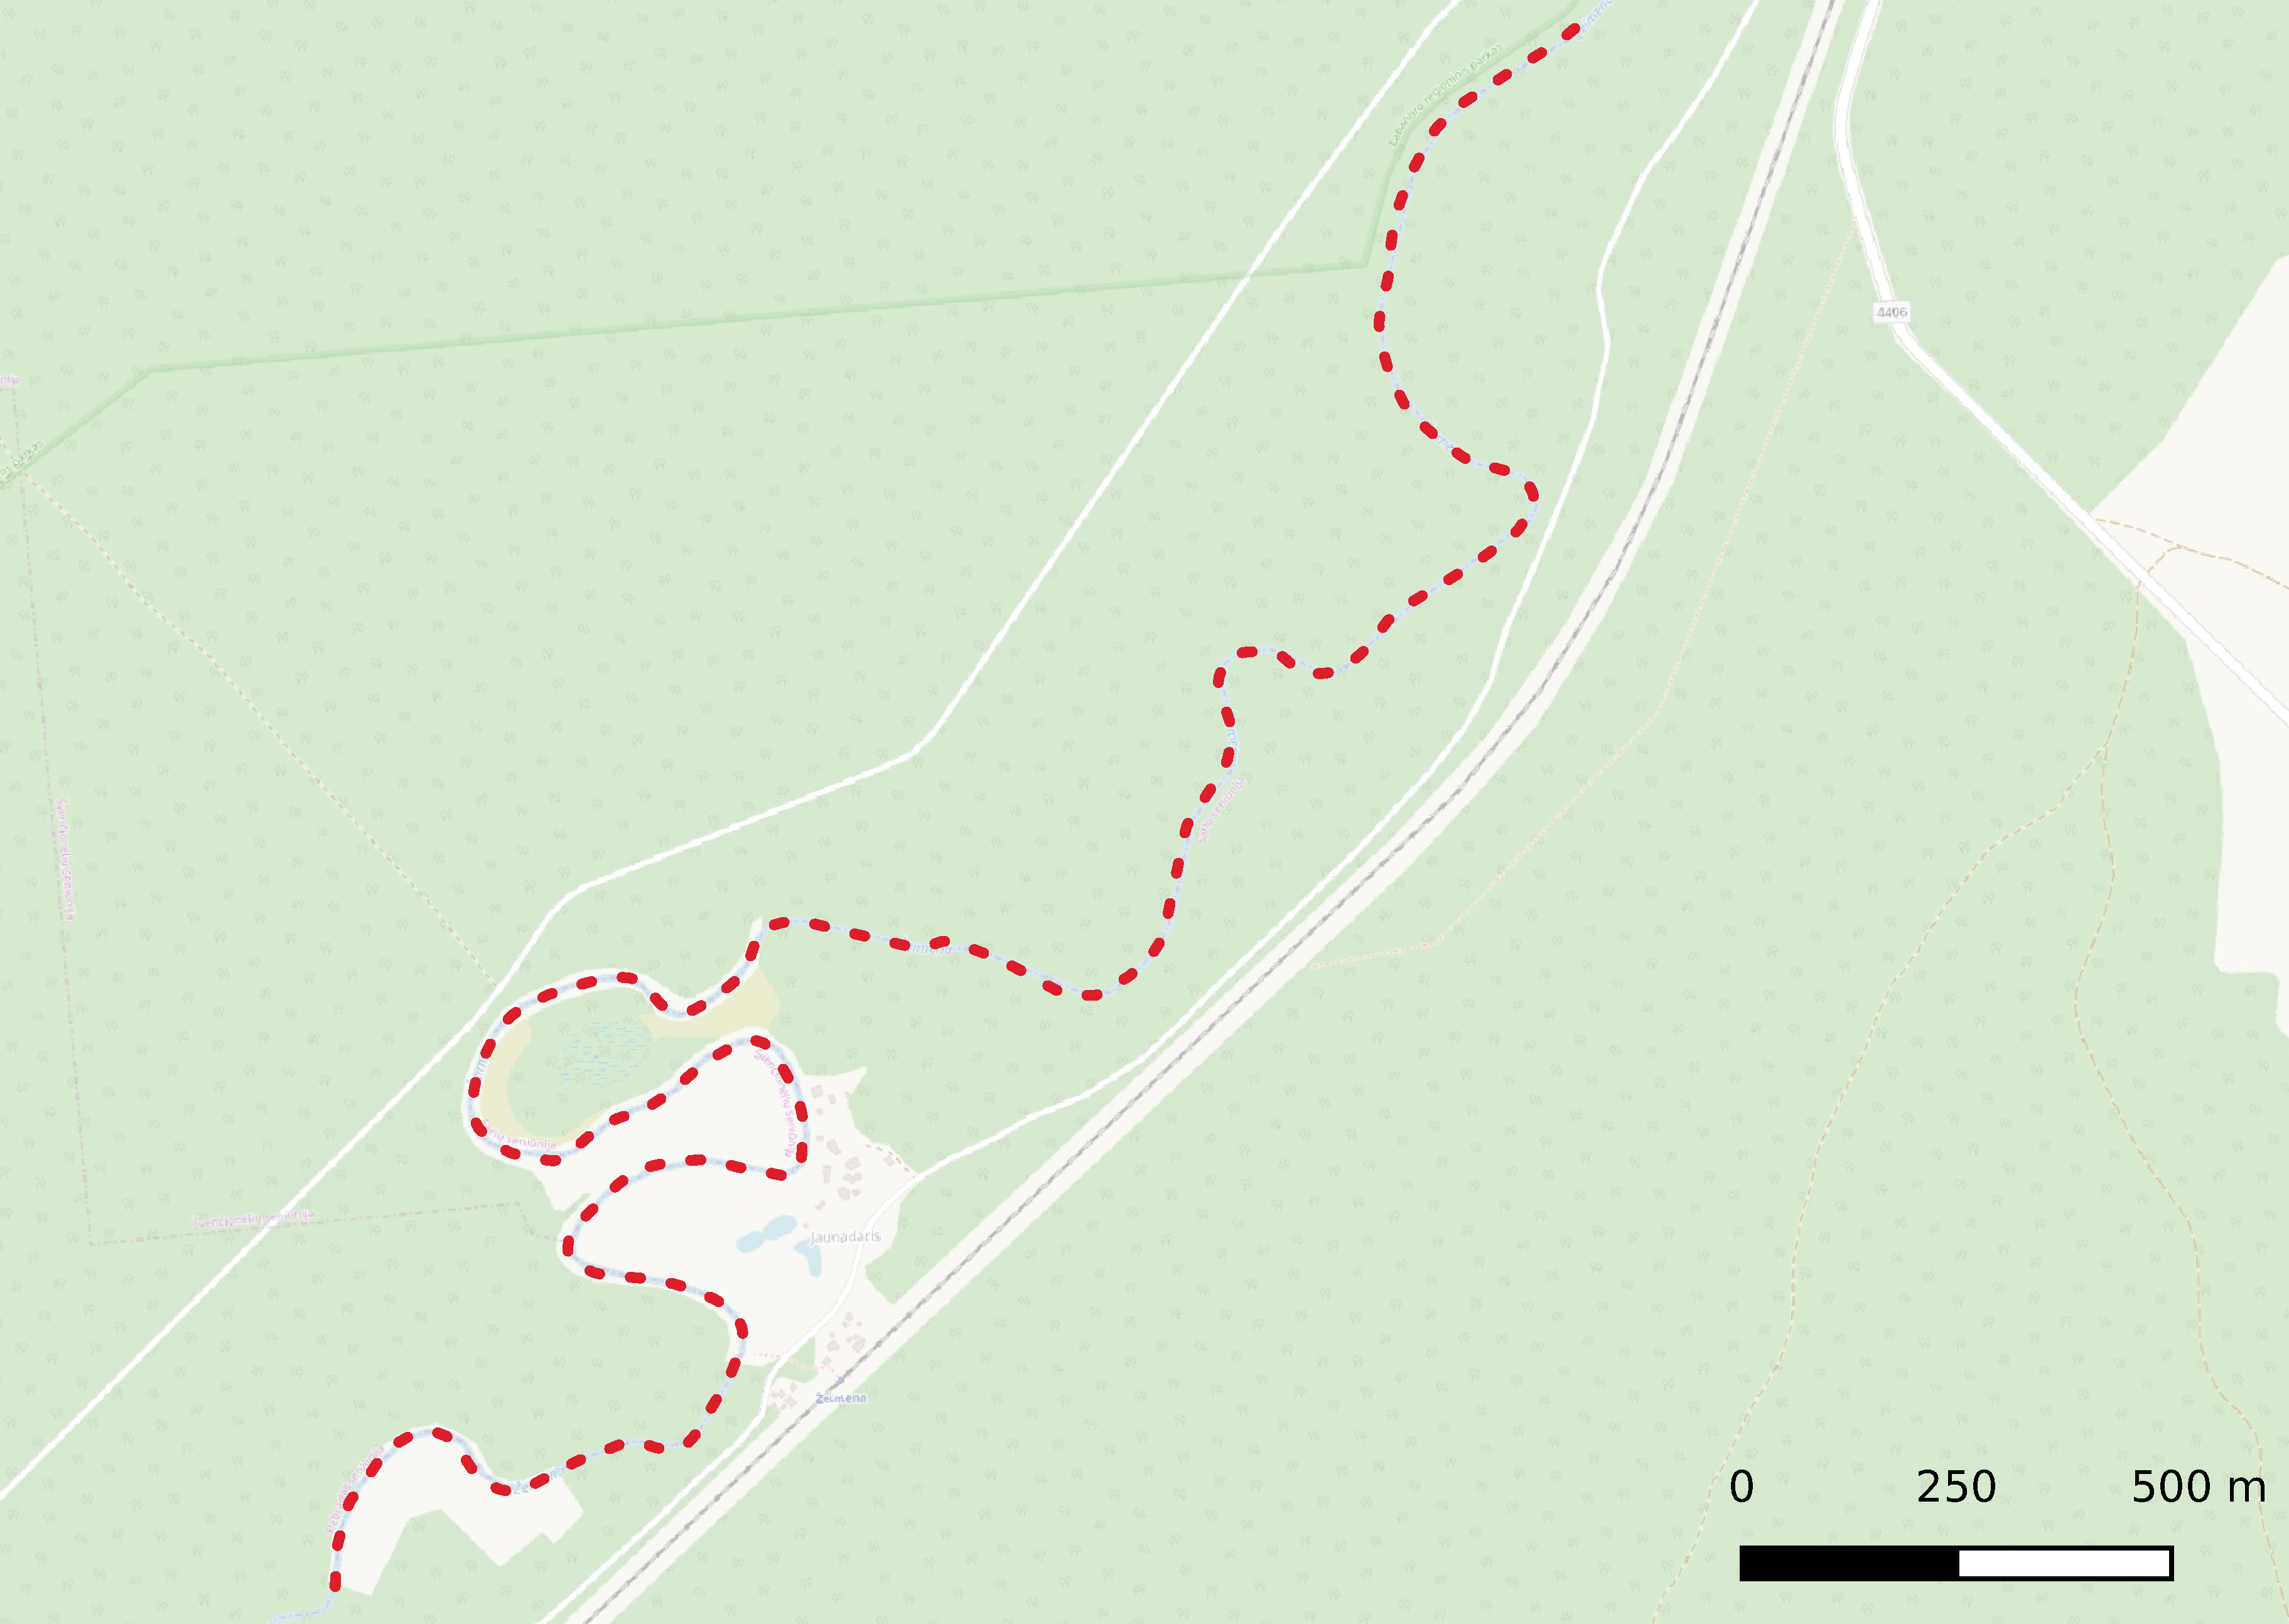
\includegraphics[width=\linewidth]{zeimena} &
    foo                                         \\ \hline
\end{tabularx}

\begin{figure}
    \centering
    \begin{subfigure}[b]{0.23\textwidth}
        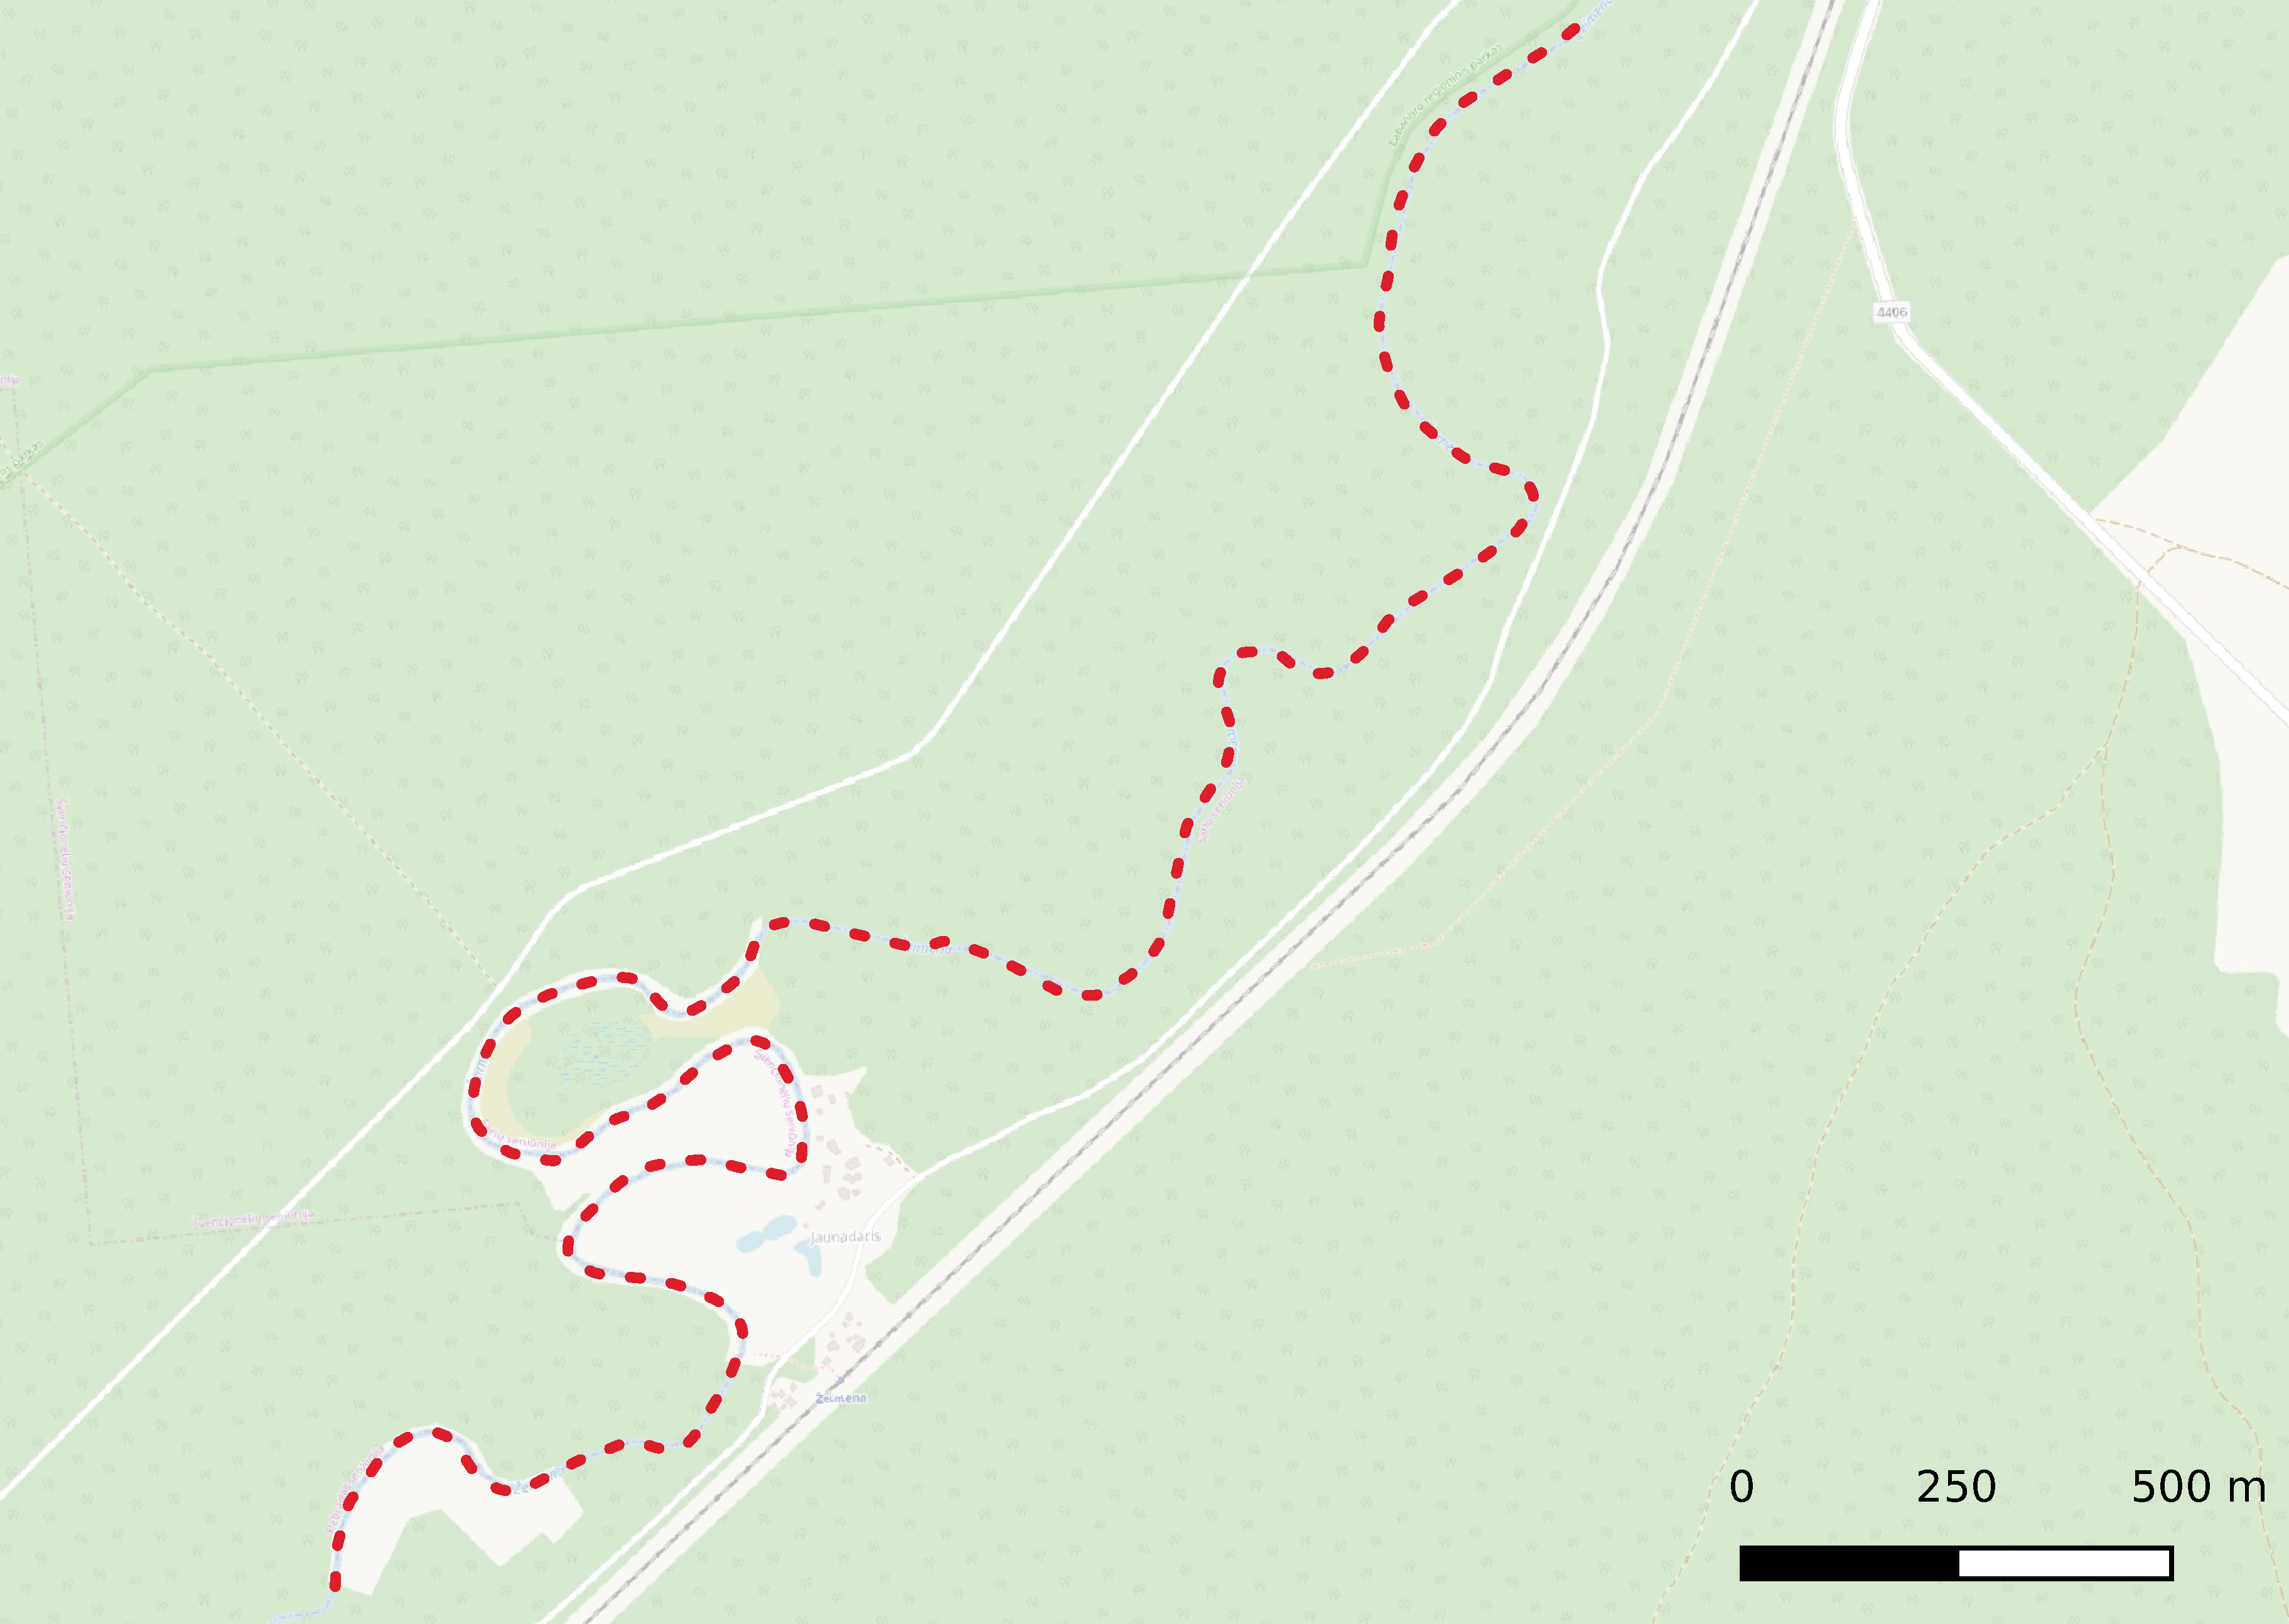
\includegraphics[width=\textwidth]{zeimena}
        \caption{original}
        \label{fig:zeimena-original}
    \end{subfigure}
    ~
    \begin{subfigure}[b]{0.23\textwidth}
        \includegraphics[width=\textwidth]{douglas-300}
        \caption{300m}
        \label{fig:douglas-300}
    \end{subfigure}
    ~
    \begin{subfigure}[b]{0.23\textwidth}
        \includegraphics[width=\textwidth]{douglas-500}
        \caption{500m}
        \label{fig:douglas-500}
    \end{subfigure}
    ~
    \begin{subfigure}[b]{0.23\textwidth}
        \includegraphics[width=\textwidth]{douglas-1000}
        \caption{1000m}
        \label{fig:douglas-1000}
    \end{subfigure}
    \caption{Douglas \& Peucker line simplifications with different tolerances}
    \label{fig:douglas-peucker}
\end{figure}

\section{Algorithms based on cartographical knowledge}

For further investigation:
\begin{itemize}
    \item \cite{jiang2003line}
    \item \cite{dyken2009simultaneous}
    \item \cite{mustafa2006dynamic}
    \item \cite{nollenburg2008morphing}
\end{itemize}

\section{My Idea}
\label{sec:my_idea}

\section{Related Work}
\label{sec:related_work}

\cite{stanislawski2012automated} studied different types of metric assessments,
such as Hausdorff distance, segment length, vector shift, surface displacement,
and tortuosity for the generalization of linear geographic elements. This
research can provide references to the appropriate settings of the line
generalization parameters for the maps at various scales.

\section{Conclusions and Further Work}
\label{sec:conclusions_and_further_work}

\printbibliography

\end{document}
